\chapter{Introducere}

\paragraph{} In this paper, we will showcase different methods of numerical integration for highly oscillating functions. These types of functions are particularly difficult to compute because, due to their steep oscillatory nature, they cannot be properly approximated using traditional methods.

We approach this challenging topic making use of the Filon quadrature, named so for, which is a more than appropriate method for rapidly oscillating functions such as
\begin{figure}[h]
    \centering
    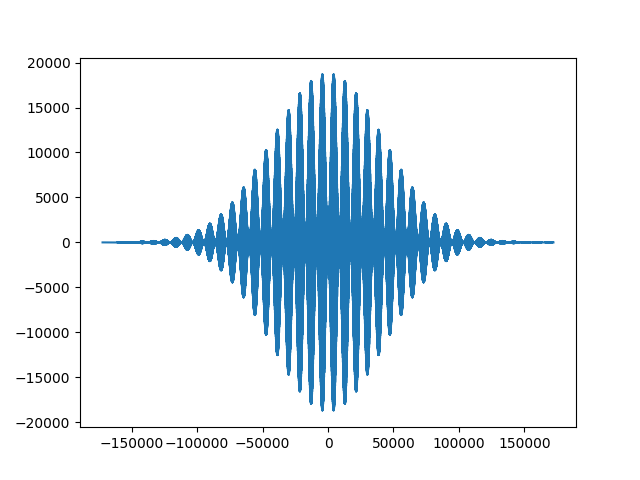
\includegraphics[scale=0.7]{c1/Figure_1.png}
    \caption{An example function}
    \label{fig:my_label}
\end{figure}

These type of "unusual" functions can be found, perhaps unsurprisingly, in a wide array of applications such as laser and radiation applications \cite{book1}, electrical engineering \cite{circ} \cite{circ2}, Quantum Field theory \cite{world}, far-field theory in aerodynamics\cite{aer} and, of course, mathematics\cite{rules} \cite{fcc} \cite{comp}. 

The pervasiveness of highly oscillating integrals that need solving definitely raises our interest in the Filon quadrature since it is a relatively straightforward and simple method that is taylor-made exactly for this type of difficult integrals.%%%Local Variables:
%%% mode: latex
%%% TeX-master: "../th"
%%% End:
